
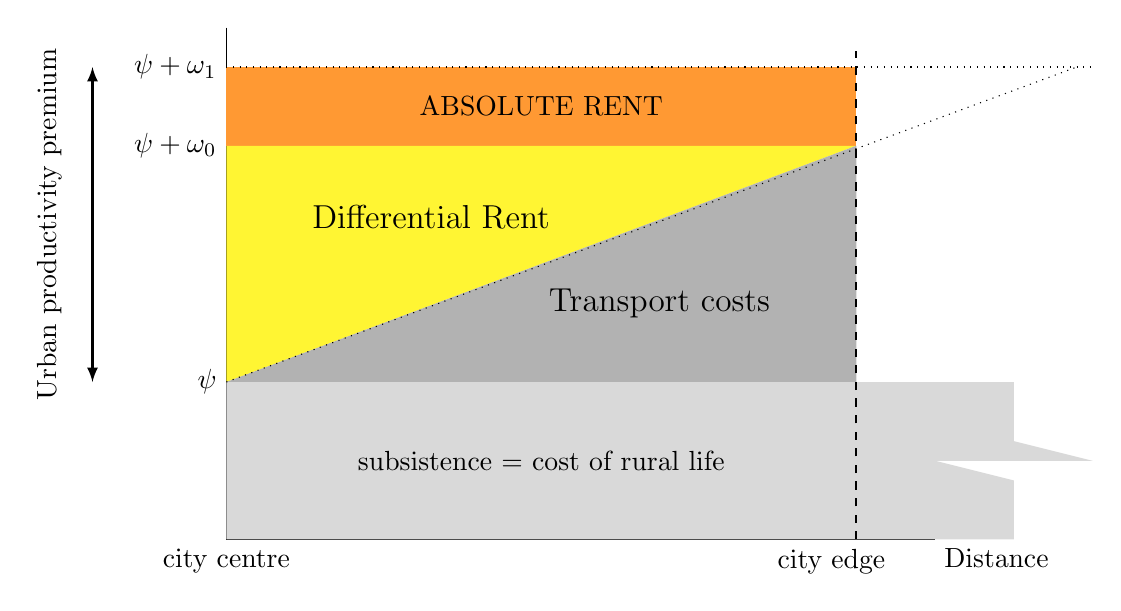
\begin{tikzpicture}[domain=0:2]
%\draw[thick,color=gray,step=.5cm, dashed] (-0.5,-.5) grid (12,5);

\draw[line width=.01 ] (1,6.5) -- (1,0)node  [below] {city centre}--(10,0) node[below right] {Distance};
%\draw[line width=.01, green ] (0,0) -- (10,0) node[right ] {Distance};
\node[below,text width=2cm]at (9,0) {city edge};

\fill [orange!80]  (1,5) --(1,6)--(9,6) --(9,5)--cycle;
\fill [yellow!80]  	(1,2) --(9,5)--(1,5) --cycle;
\fill [gray!60] 	(9,5) --(1,2)--(9,2) --cycle;
\fill [gray!30] 	(1,0) --(1,2)--(11,2) --(11,1.25)-- (12,1)-- (10,1)--(11,.75)--(11,0)--cycle;



\node	at 	(1,5)[left]{$\psi +\omega_0$} ;
\node	at 	(1,6)[left]{$\psi +\omega_1$} ;
\node	at 	(1,2)[left]{$\psi$} ;

\draw[thick , dashed] (9,0)  -- (9,6.2); 
\draw[dotted] (1,6)  -- (12,6); 
\draw[dotted] (1,2)  -- (11.8,6); 

%\draw[thick,color=red] (1.5,0) -- (1.5,1) node[below right] {Fixed cost} -- (1.5,1.5) --(10,3.25)node[above left] {total cost};

\node at (5,5.5)[] 	{ABSOLUTE RENT} ;
\node  at (6.5,3)	{\large Transport costs};
\node  at (3.6,4.1)	{\large  Differential Rent};
\node at (5,1)[] {subsistence = cost of rural life} ;
\node at (-1.25,4)[rotate=90] {Urban productivity premium} ;
\draw[thick,latex-latex] (-.7,2) -- (-.7,6) ;
\end{tikzpicture} 
